\documentclass[12pt,letterpaper,oneside]{report}
\usepackage{fullpage,setspace,url,amsmath}
\usepackage{graphicx}
\usepackage{amssymb}
\usepackage[left=1in,right=1in,top=1in,bottom=1in]{geometry}

%%% Commands
\newcommand \groupname{Team Fuzzy Wuzzy}

\newcommand \arfa{$\alpha$}
\newcommand \code[1]{\texttt{#1}}
\newcommand \TODO[1]{\textbf{#1}}
\newcommand \qq[1]{``{#1}''}
\newcommand \etal{\textit{et al.}}

\renewcommand{\thesection}{\arabic{section}}


%%% Style
%bibliographystyle{ieeetr}
\usepackage[colorlinks=true, urlcolor=black, linkcolor=black, citecolor=black]{hyperref}


%%% Metadata
\title{Self-Organizing Map Character Recognizer}

%\subtitle{\groupname}
\author{ David Briscoe }


%%% Document
\begin{document}

% Front matter
\pagenumbering{roman}
\setcounter{page}{1}
%\setstretch{2}
\maketitle
\tableofcontents
\clearpage

% Main matter
\setcounter{section}{0}
\pagenumbering{arabic}
\setcounter{page}{1}



\section{Introduction}
% Explain some problem statements stuff here.
The purpose of this project was to develop a self-organizing map that would train on a selection of characters with different font faces and cluster them into groups corresponding to each letter. We will only consider the letters A to F.

\section{Objectives}
% State objectives of the project in excruciating detail, yay!
% Opportunities for citing references in absurd and wonderful ways?

\begin{enumerate}
\item Produce some input data.
\item Provide a system to ensure the input data is the same form-factor so it can be accepted by the self-organizing map.
\item Create an implementation of a self-organizing map that accepts a list of variables for inputs.
\item Create a GUI that would allow the user to select an image of a letter to input into the self-organizing map and to display the output cluster.
\end{enumerate}

\clearpage
\section{Design and Implementation}
\subsection{Data and Data Normalization}
The input data are the letters A to F for three fonts. The fonts were selected at random, but novelty fonts were excluded. The fonts are Deja Vu Sans, Nimbus Roman, and Times New Roman. 

The fonts were taken from a word processor at 12 pt font and at 300\% zoom using a screen capture as shown in Figure \ref{fig:font-screengrab}. Each letter was separated and cropped to include no surrounding whitespace.

\begin{figure}[ht]
  \centering
  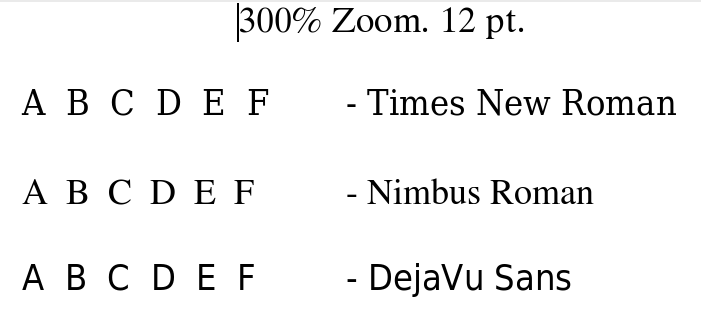
\includegraphics[width=5in]{diagrams/font-screengrab}
  \caption{The source for the fonts.}
  \label{fig:font-screengrab}
\end{figure}

After this process, the inputs were roughly similar in size, but each pixel is
represented by an RGB value. The RGB value provided more information than
necessary since the images contained no colour, and the images had to be the
exact same dimensions. These issues were fixed by running them through
\code{normalize.py} (\textit{see also README.txt}). This program converted
them to greyscale and stretched them to all be the same size.


\subsection{Self-organizing map}
% Describe membership functions and how they were implemented in code
The self-organizing map is very straightforward. It contains a weight for each cluster. Each weight has the same number of elements as each input.

When training the self-organizing map, Euclidean distance is used to determine which weight is \qq{closest} to the input.


\subsection{Graphical User Interface}
% Describe the interface
The interface displays what the current input looks like and the current output of the self-organizing map. There are buttons to train the self-organizing map and to reset it back to its original (randomized) state. Figure \ref{fig:gui-plain} shows the interface.

\begin{figure}[ht]
  \centering
  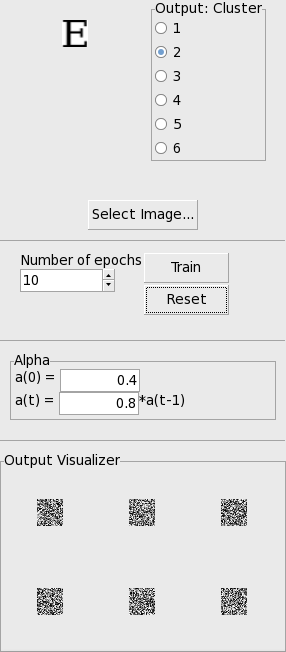
\includegraphics[width=180px]{diagrams/gui-plain} 
  \caption{The graphical user interface for inputting data into the self-organizing map. This screen shows the system initialized with random weights.}
  \label{fig:gui-plain}
\end{figure}

The output displays the cluster that the self-organizing map has selected for the input image. The same input letter (with different or the same font face) should have the same cluster for its output.

The user can select a new image for input or train the self-organizing map.

Training will take all of the images in the \code{data} folder and pass them into the self-organizing map for the user's input number of epochs. The $\alpha(t)$ function used for training is displayed in the middle of the GUI. The user can modify $\alpha(0)$ or change the factor $k$ in $\alpha(t) = k\alpha(t-1)$ (how much \arfa~is scaled by on each training epoch). 

Finally, the bottom of the window displays the 6 clusters visualized as images. Each image represents the elements in the weight for that cluster and they are laid out to look like the input images. This visualizer makes it easier to see how each weight compares to the input letter.

\subsection{Additional Output}
During training, there is additional output on the command-line to facilitate tuning. On each epoch, the self-organizing map prints out the number of inputs that match each cluster. The following output shows three clusters modified for that training epoch.
\begin{verbatim}
(cluster number,number of matching inputs): [(0, 7), (1, 8), (5, 3)]
\end{verbatim}

\subsection{Training the System}
Training the system can be done through the user interface. The output visualizer and the additional epoch output can be used to determine the effectiveness of training. Additionally, the system uses a constant seed for the random number generator that initializes the weights so that all tests will use the same initial values. This allowed repeatability and removes a lot of guess work in testing. However, the inputs to the self-organizing map are selected at random so each training session may be different.

\subsection{Testing the System}
The user can select images to input into the system. The system will output a cluster in the range [1-6] that characterizes the image. The same letter (even in different font faces) should output the same cluster number.

\clearpage
\section{Analysis}
% Analyze the results of our project...


\subsection{Initial Tests}
I tried small values for $\alpha(0)$: $\alpha(0) = 0.001, 0.01, 0.1$, but none of these values resulted in more than two weights being modified. The random values resulted in only one or two weights that are close to the appearance of the letters, and since the $\alpha(0)$ value is so small, very little change resulted (even with large epochs).

\subsection{Training the System}
Trying larger values for $\alpha(0)$, I used $\alpha(0) = 1.0$ and $\alpha(t) = 0.8\alpha(t-1)$ and 10 epochs. This produced three clusters: 
\begin{verbatim}
(cluster number,number of matching inputs): [(0, 7), (1, 8), (5, 3)]
\end{verbatim}

The output visualizer shown in Figure \ref{fig:first-test} showed that the letter A was being captured very well, but all other letters were being grouped into only two other categories.

\begin{figure}[ht]
\centering
  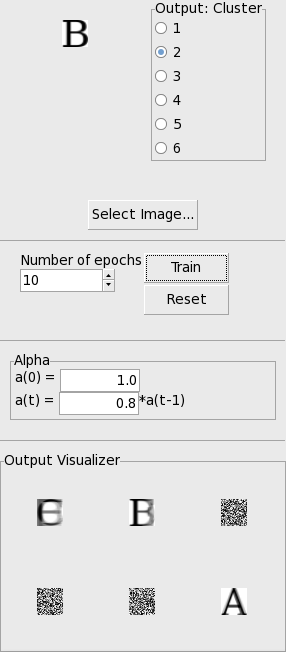
\includegraphics[width=180px]{diagrams/first-test.png} 
  \caption{The output visualizer results for the first test.}
  \label{fig:first-test}
\end{figure}

Training for another 10 epochs resulting in another cluster being formed. Figure \ref{fig:second-test} illustrates how the new cluster strongly characterized C.

\begin{figure}[ht]
\centering
  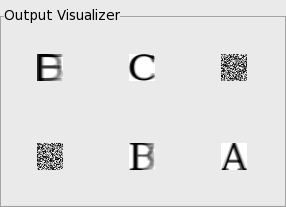
\includegraphics[width=180px]{diagrams/second-test.png} 
  \caption{The output visualizer results for the second test.}
  \label{fig:second-test}
\end{figure}

The first cluster appeared to characterize E most strongly but also B and D. The fifth cluster characterized F strongly but also characterized B and D.

Training a third time swapped the first and fifth clusters.

\begin{figure}[ht]
\centering
  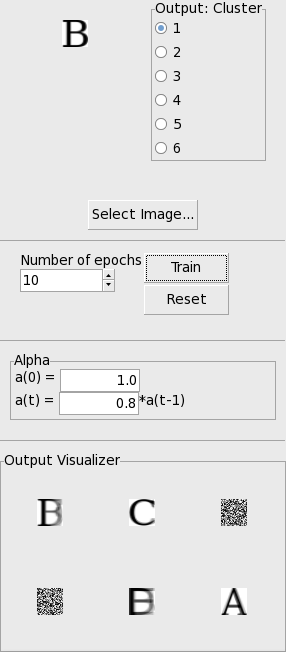
\includegraphics[width=180px]{diagrams/third-test.png} 
  \caption{The output visualizer results for the third test.}
  \label{fig:third-test}
\end{figure}

At this point, the system appeared to make no further progress in training. This iteration was a failure, so I discarded this data and tried again.

\subsection{Improved Results}
After several more attempts at training, the self-organizing map produced some good results. One one test, it produced five clusters after 10 epochs. The output visualizer in Figure \ref{fig:good-test} illustrates how A, C, and D are well captured by the system. E and F are strongly captured, but mixed with B and D.

\begin{figure}[ht]
  \centering
  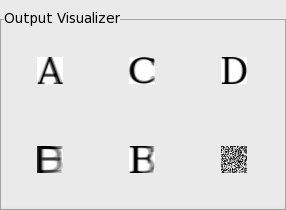
\includegraphics[width=180px]{diagrams/good-test.png} 
  \caption{The output visualizer results for the good test.}
  \label{fig:good-test}
\end{figure}

Running tests produced the following results:
\begin{itemize}
    \item\textbf{{A:}} All fonts for the letter A were grouped as output 1.
    \item\textbf{{B:}} Both of the Roman fonts grouped B as 5, but the sans serif font (Deja Vu Sans) was grouped as 4.
    \item\textbf{{C:}} All fonts for the letter grouped as output 2.
    \item\textbf{{D:}} Roman fonts grouped as 3, but the sans serif font grouped as 4.
    \item\textbf{{E:}} Roman fonts grouped as 5, but the sans serif font grouped as 4.
    \item\textbf{{F:}} Roman fonts grouped as 5, but the sans serif font grouped as 4.
\end{itemize}

\subsection{Alternative Initial Weights}
In an attempt to improve the character recognition, I changed the way weights are initialized. One attempt was to make the initial values of the weights to have zero distance to the sets of letters for one font face. This produced a near perfect recognizer, even with the differences between roman and sans serif fonts. Figure \ref{fig:perfect-test} illustrates the output visualizer for this self-organizing map.

\begin{figure}[ht]
  \centering
  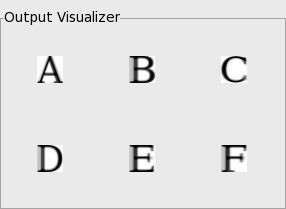
\includegraphics[width=180px]{diagrams/perfect-test.png} 
  \caption{The output visualizer results for the perfect test.}
  \label{fig:perfect-test}
\end{figure}

\section{Conclusions}
The self-organizing map is clearly useful in recognizing characters. However, it has difficulty separating very similar characters. In this regard, the self-organizing map suffers from the use of unsupervised learning. Since the self-organizing map has no information to distinguish an E from an F except for its past experiences, the two blend together and result in a common cluster. Distinct characters like A and C, on the other hand, are well captured by the self-organizing map. 

It is not useful to use small values for $\alpha(0)$. Using a larger value helps to create clusters quickly, but may train the self-organizing map too quickly on certain letters.

\section{Recommendations}
Due to the self-organizing map's difficulty in separating some similar letters, some investigation into different techniques would be beneficial. Given the nature of the problem, it would be useful to use a supervised learning technique. We know each letter that we input, so we could provide the target data as well as the input data.

The output for this self-organizing map was only six clusters, but it could be expanded to include more clusters. Having multiple clusters for each letter could help prevent multiple letters from being mapped to one cluster. Additionally, a neighbourhood function could be introduced to spread the effect of each match across the different weights.

The initialization of the weights in the self-organizing map could be changed to find a better initial situation to match the letters against. Initializing the weights to match one of the inputs seems promising and it should be tested with a wider variety of font faces.

Finally, I would recommend expanding this solution to use the full alphabet and a greater number of fonts. I think that it would be interesting to see how many letters are confused and what extra preprocessing can be done to improve the recognition. Preprocessing filters such as sharpening the image (to increase the contrast), blurring the image (to increase the size of the gradient), and converting the image to black and white (instead of greyscale) offer interesting possibilities.

\clearpage
\section{Appendix: Starting and Running the Application}\label{apx:running}
The application can be run as an executable using \texttt{python} at the command line.
Note that my application requires Python 2.5 and some python libraries: PIL and wxpython.

\subsection{Starting the Python Application}
\begin{enumerate}
  \item There are some dependencies required: python, wxpython, and PIL. Instructions for installing these can be found in README.txt in the Dependencies section.
  \item On a Windows system, open the \code{runapplication.bat} script. On a
      Unix-like system, open the \code{runapplication.sh} script.
  \item For more information see the README.txt file.
\end{enumerate}

% Back matter
%\bibliography{ref}

\end{document}
